\section{Introduzione}
Un programma eseguito su un'architettura dotata di una singola unità di elaborazione centrale (CPU) può essere eseguita esclusivamente in maniera sequenziale (un'istruzione alla volta) in figura \ref{fig:single-computation}
% TODO: \usepackage{graphicx} required
\begin{figure}[th]
	\centering
	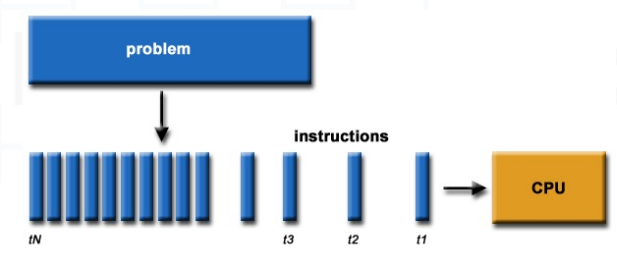
\includegraphics[width=0.7\linewidth]{img/single-computation}
	\caption{esecuzione su un'architettura dotata di una sola CPU.}
	\label{fig:single-computation}
\end{figure}
